\chapter{Metric learning}


\begin{description}
    \item[Metric learning] \marginnote{Metric learning}
        Task of training a network that produces discriminative embeddings (i.e., with a clustered structure) such that:
        \begin{itemize}
            \item The distance of related objects (i.e., intra-class distance) is minimized.
            \item The distance of different objects (i.e., inter-class distance) is maximized.
        \end{itemize}
\end{description}

\section{Face recognition}

\begin{description}
    \item[Face recognition] \marginnote{Face recognition}
        Given a database of identities, classify a query face.

        \begin{description}
            \item[Open-world setting]
                System where it is easy to add or remove identities.
        \end{description}
\end{description}


\subsection{Face recognition as classification}

\begin{description}
    \item[Plain classifier] \marginnote{Plain classifier}
        Consider each identity as a class and use a CNN with a softmax head to classify the input image.

        \begin{remark}
            This approach requires a large softmax and do not allow adding or removing identities without retraining.
        \end{remark}

    \item[kNN classifier] \marginnote{kNN classifier}
        Use a feature extractor to embed faces and use a kNN classifier to recognize it.

        \begin{description}
            \item[Gallery] \marginnote{Gallery}
                Set of embeddings of known identities.
        \end{description}

        \begin{remark}
            This approach allows to easily add or remove new identities.
        \end{remark}

        \begin{figure}[H]
            \centering
            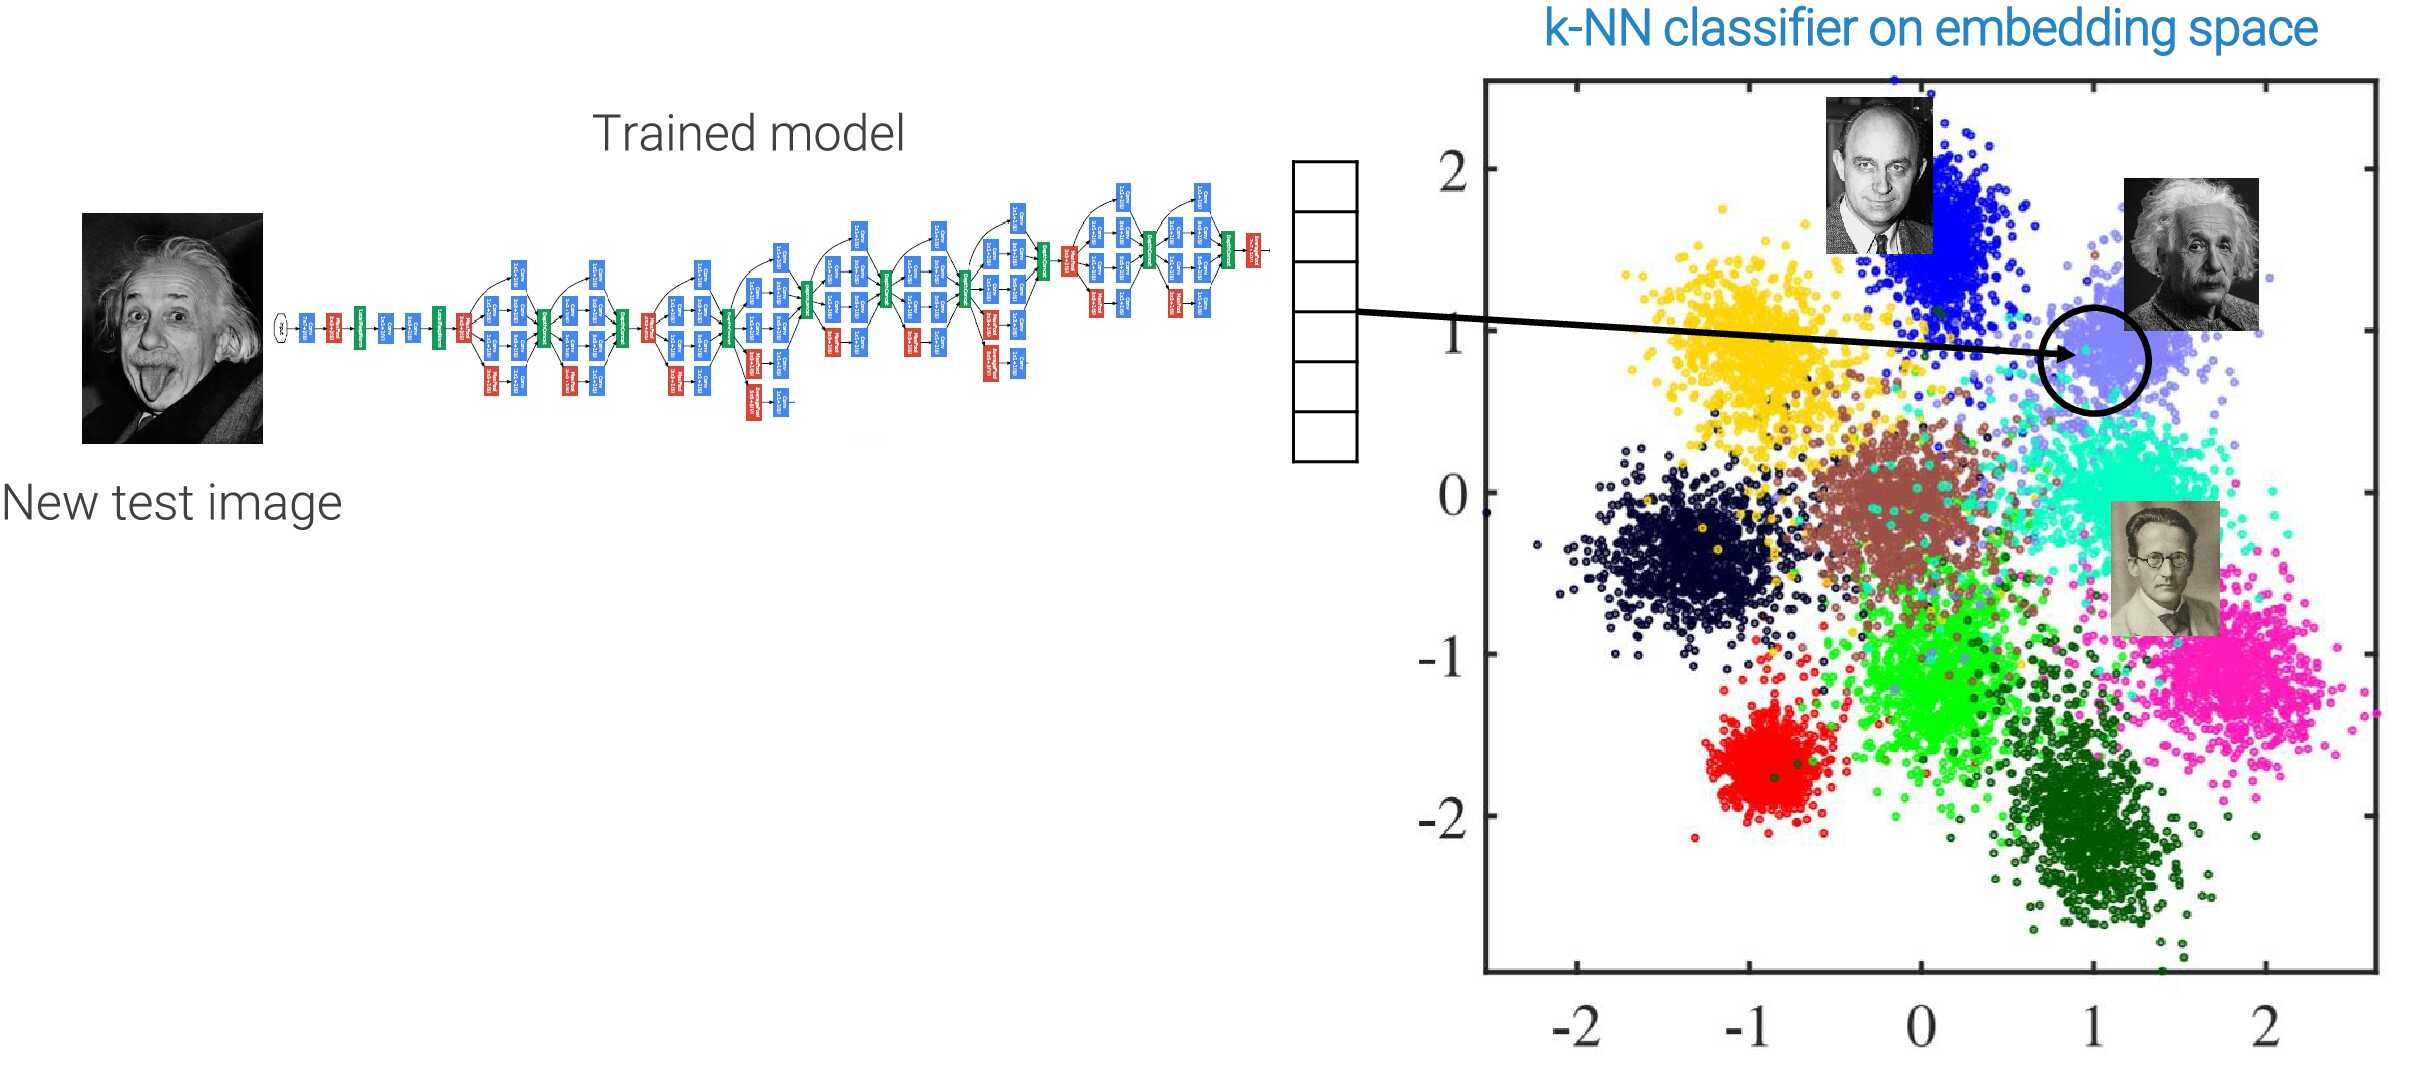
\includegraphics[width=0.7\linewidth]{./img/_cnn_knn_face_recognition.jpg}
        \end{figure}

        \begin{remark}
            Feature extractors for classification are trained using the cross-entropy loss to learn semantically rich embeddings. However, when classifying, these embeddings are passed through a final linear layer. Therefore, it is sufficient that they are linearly separable.

            In other words, the distance between elements of the same class can be arbitrarily large and the distance between different classes can be arbitrarily small, as long as they are linearly separable.

            \begin{figure}[H]
                \centering
                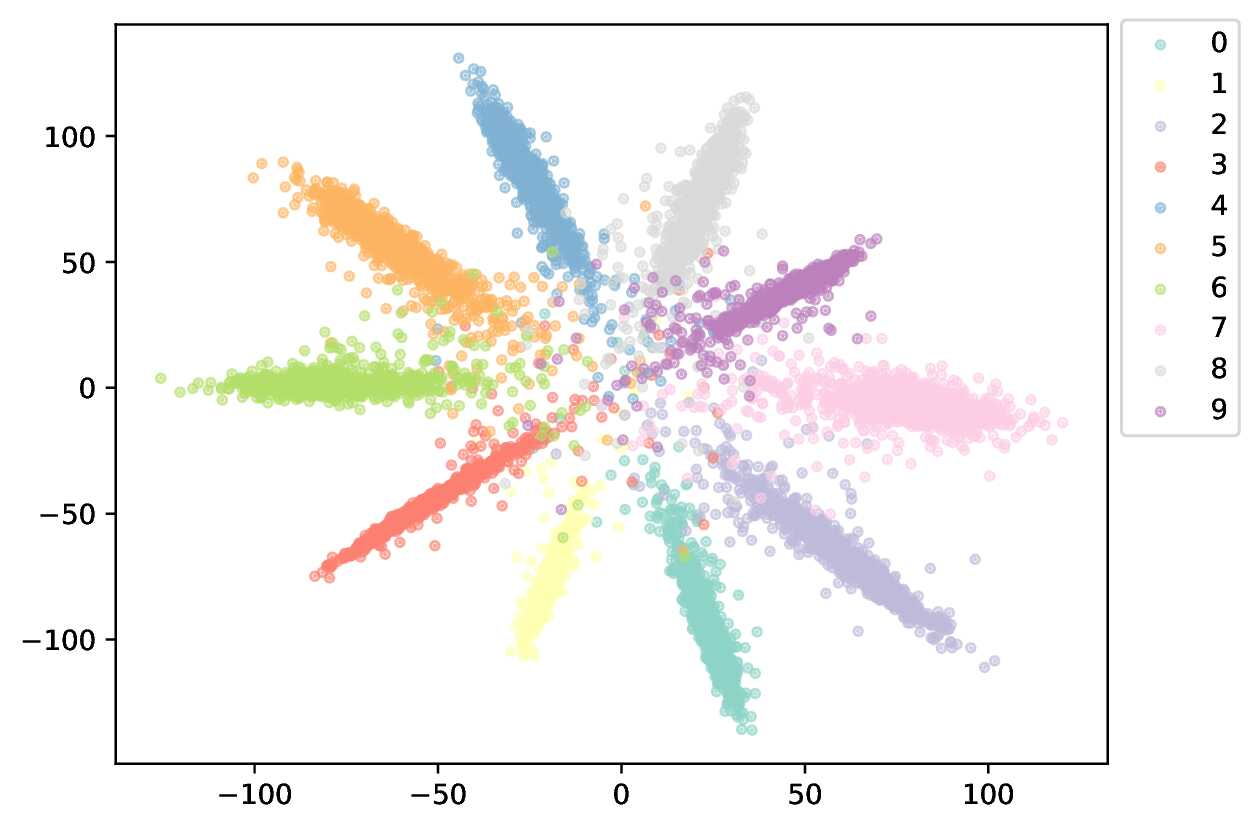
\includegraphics[width=0.45\linewidth]{./img/_mnist_embeddings.jpg}
                \caption{MNIST embeddings in 2D}
            \end{figure}
        \end{remark}
\end{description}



\section{Metric learning losses}

\begin{description}
    \item[Face verification] \marginnote{Face verification}
        Task of confirming that two faces represent the same identity. This problem can be solved by either:
        \begin{itemize}
            \item Using better metrics than the Euclidean distance (e.g., as done in DeepFace).
            \item Using better embeddings (e.g., as done in DeepID or FaceNet).
        \end{itemize}

        \begin{remark}
            This task can be used to solve face recognition.
        \end{remark}
\end{description}


\subsection{Contrastive loss}

\begin{description}
    \item[Siamese network training] \marginnote{Siamese network training}
        Train a network by comparing its outputs from two different inputs. This can be virtually seen as training two copies of the same network with shared weights.

        \begin{figure}[H]
            \centering
            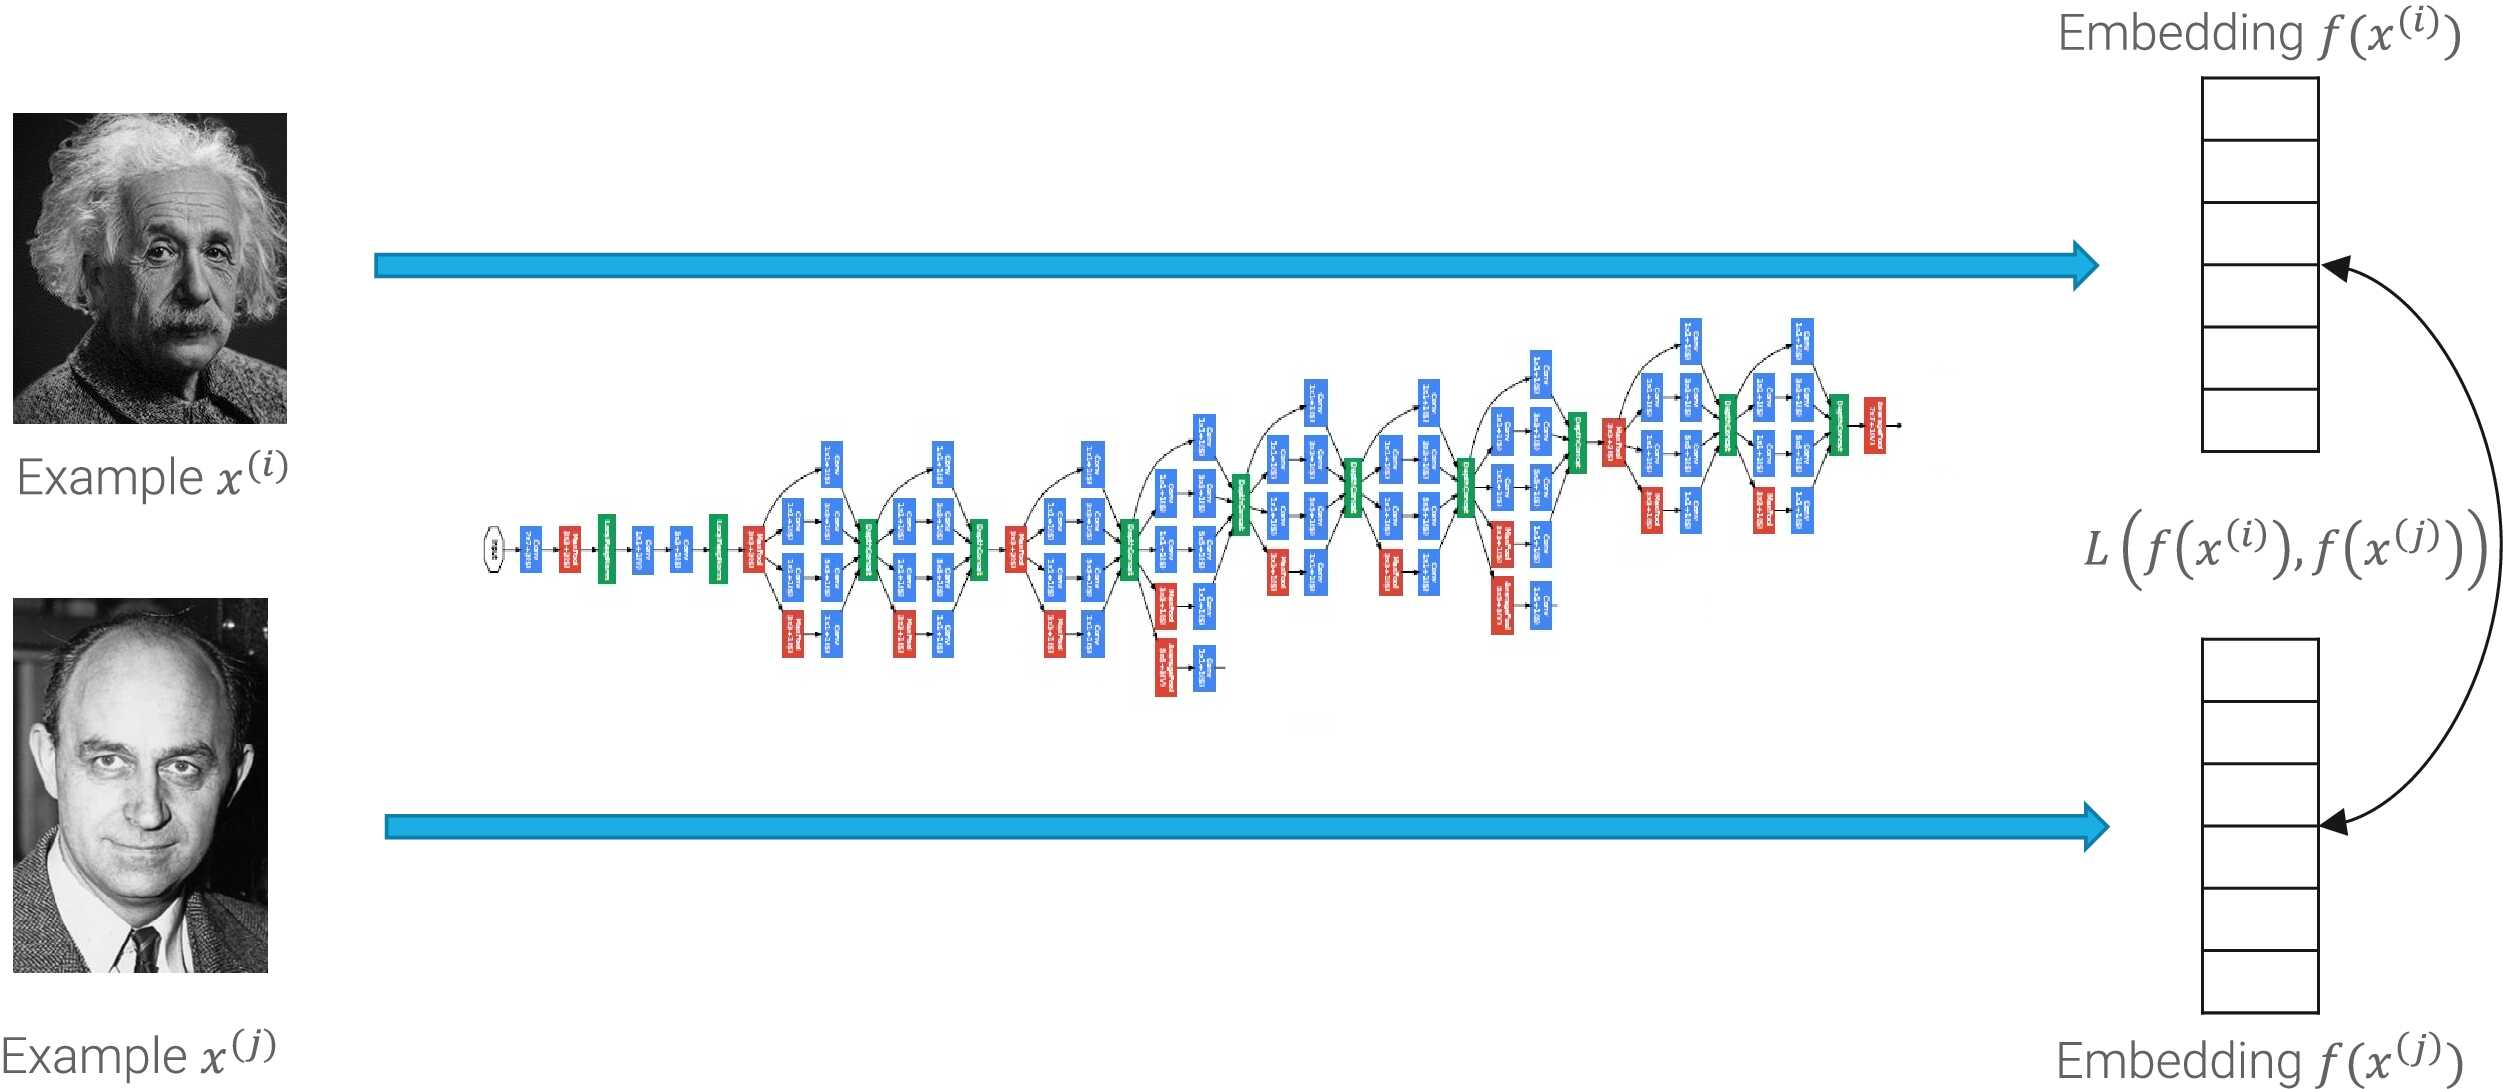
\includegraphics[width=0.7\linewidth]{./img/_siamese_network.jpg}
        \end{figure}

        \item[Contrastive loss] \marginnote{Contrastive loss}
            Loss to enforce clustered embeddings. It is defined as follows:
            \[
                \mathcal{L}\left( f(x^{(i)}), f(x^{(j)}) \right) = 
                \begin{cases}
                    \Vert f(x^{(i)}) - f(x^{(j)}) \Vert_2^2 & \text{if $y^{(i, j)} = +1$ (i.e., same class)} \\
                    - \Vert f(x^{(i)}) - f(x^{(j)}) \Vert_2^2 & \text{if $y^{(i, j)} = 0$} \\
                \end{cases}
            \]
            As the second term is not lower-bounded (i.e., it can be arbitrarily small), a margin $m$ is included to prevent pushing different classes too far away:
            \[
                \begin{split}
                    &\mathcal{L}\left( f(x^{(i)}), f(x^{(j)}) \right) = 
                    \begin{cases}
                        \Vert f(x^{(i)}) - f(x^{(j)}) \Vert_2^2 & \text{if $y^{(i, j)} = +1$} \\
                        \max\left\{0, m - \Vert f(x^{(i)}) - f(x^{(j)}) \Vert_2\right\}^2 & \text{if $y^{(i, j)} = 0$} \\
                    \end{cases} \\
                    &= y^{(i, j)} \Vert f(x^{(i)}) - f(x^{(j)}) \Vert_2^2 + (1-y^{(i, j)}) \max\left\{0, m - \Vert f(x^{(i)}) - f(x^{(j)}) \Vert_2\right\}
                \end{split}
            \]

            \begin{remark}
                A margin $m^+$ can also be added to the positive branch to prevent collapsing all embeddings of the same class to the same point.
            \end{remark}

            \begin{remark}
                The negative branch $\max\left\{0, m - \Vert f(x^{(i)}) - f(x^{(j)}) \Vert_2\right\}$ is the hinge loss, which is used in SVM.
            \end{remark}

            \begin{remark}
                With L2 regularization, the fact that the second term is not lower-bounded is not strictly a problem as the weights lay on a hyper-sphere and therefore set a bound to the output. Still, there is no need to push the embeddings excessively far away.
            \end{remark}

    \item[DeepID2] \marginnote{DeepID2}
            CNN trained using contrastive and cross-entropy loss.

            \begin{description}
                \item[Test-time augmentation]
                    The trained network is used as follows:
                    \begin{enumerate}
                        \item Process 200 fixed crops of the input image.
                        \item Select the top-25 crops.
                        \item Use PCA to reduce the concatenation of the output $4000$-dimensional vector into a $180$-dimensional embedding.
                    \end{enumerate}
            \end{description}

            \begin{figure}[H]
                \centering
                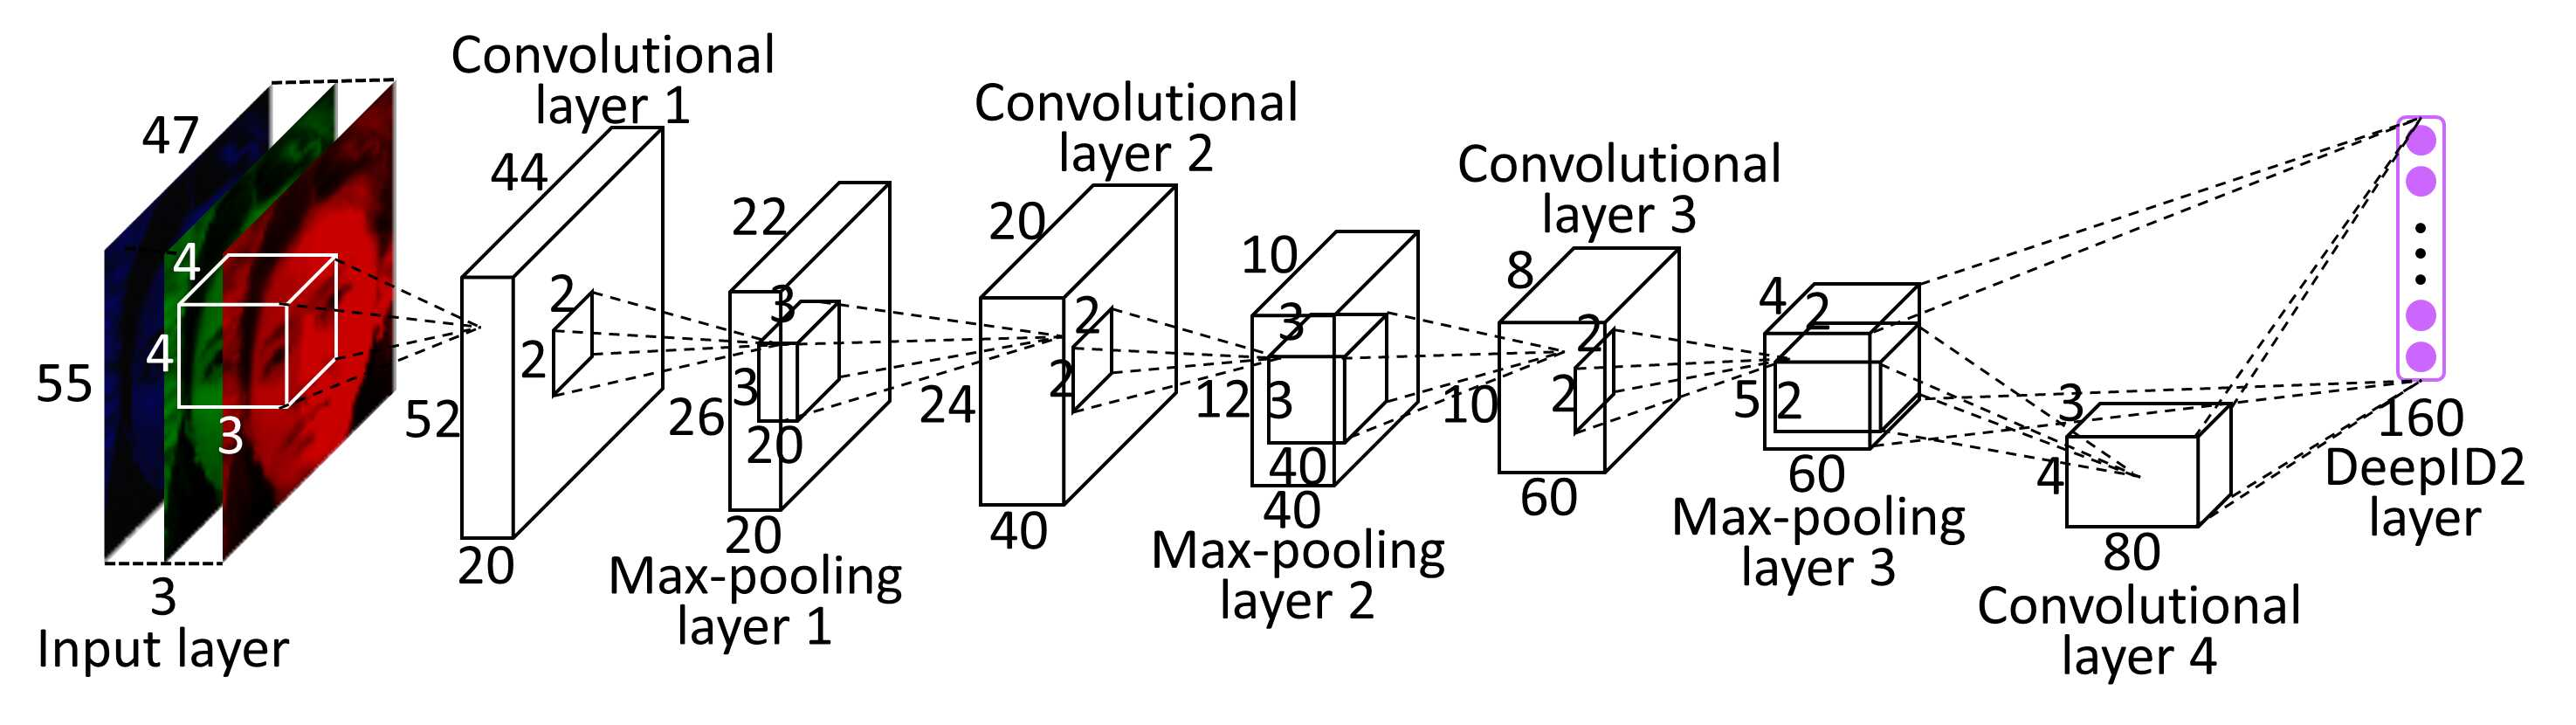
\includegraphics[width=0.7\linewidth]{./img/deepid2.jpg}
                \caption{DeepID2 on a single crop}
            \end{figure}
\end{description}

\begin{remark}
    Contrastive loss indirectly (i.e., separately) enforces that similar entities should be close and different ones should be distant.
\end{remark}


\subsection{Triplet loss} \label{sec:triplet_loss}

\begin{description}
    \item[Triplet loss] \marginnote{Triplet loss}
        Enforces at the same time that embeddings should be close for the same entity and distant for different ones.

        \begin{description}
            \item[Naive formulation] 
                Given:
                \begin{itemize}
                    \item An anchor image $A$ (i.e., reference image),
                    \item A positive image $P$,
                    \item A negative image $N$,
                \end{itemize}
                The triplet loss is defined as:
                \[ \Vert f(P) - f(A) \Vert_2^2 < \Vert f(N) - f(A) \Vert_2^2 \]

                \begin{remark}
                    This definition does not guarantee sufficient inter-class distance and also risks training collapse (i.e., constant embeddings close to 0 satisfy the loss).
                \end{remark}

            \item[Margin formulation] 
                Given a margin $m$, the triplet loss is defined as:
                \[ 
                    \begin{gathered}
                        \Vert f(P) - f(A) \Vert_2^2 + m < \Vert f(N) - f(A) \Vert_2^2 \\
                        \Vert f(P) - f(A) \Vert_2^2 - \Vert f(N) - f(A) \Vert_2^2 + m < 0 \\
                        \mathcal{L}_\text{triplet}(A, P, N) = \max \left\{ 0,  \Vert f(P) - f(A) \Vert_2^2 - \Vert f(N) - f(A) \Vert_2^2 + m \right\}
                    \end{gathered}
                \]

                \begin{figure}[H]
                    \centering
                    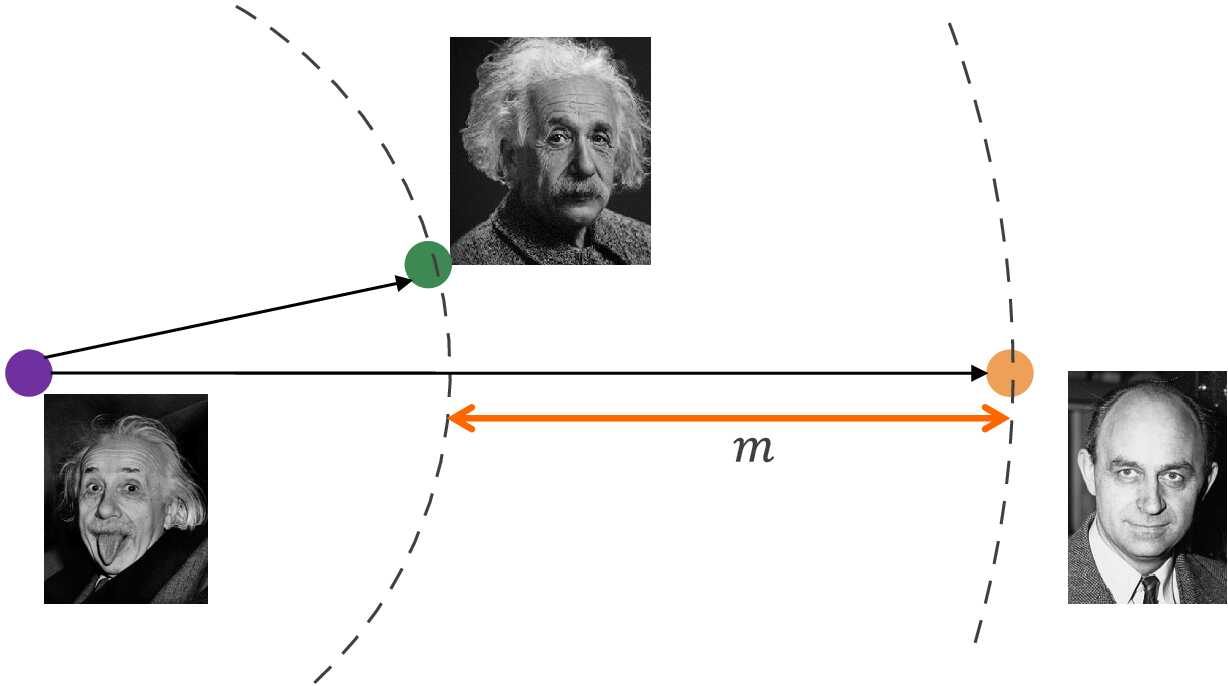
\includegraphics[width=0.45\linewidth]{./img/_triplet_loss.jpg}
                \end{figure}

                \begin{remark}
                    Differently from contrastive loss, triplet loss naturally prevents collapse using a single hyperparameter $m$.
                \end{remark}

                \begin{remark}
                    By considering an anchor, a face recognition dataset is composed of a few positive images and lots of negative images. If the embedding of a negative image is already far enough, the loss will be $0$ and does not affect training, making convergence slow.
                \end{remark}
        \end{description}

    \item[Semi-hard negative mining] \marginnote{Semi-hard negative mining}
        Given an anchor $A$, a batch of $B$ samples is formed as follows:
        \begin{enumerate}
            \item Sample $D \ll B$ identities.
            \item For each identity, sample a bunch of images.
            \item Consider all possible anchor-positive pairs $(A, P)$. Randomly sample a negative image $N$ and create a triplet $(A, P, N)$ if it is semi-hard (i.e., within the margin):
            \[ \Vert f(P) - f(A) \Vert_2^2 < \Vert f(N) - f(A) \Vert_2^2 < \Vert f(P) - f(A) \Vert_2^2 + m \]
            Repeat this process until the batch is filled.
        \end{enumerate}

        \begin{remark}
            Batches are formed on-line (i.e., during training).
        \end{remark}

        \begin{remark}
            It has been seen that hard-negatives ($\Vert f(P) - f(A) \Vert_2^2 > \Vert f(N) - f(A) \Vert_2^2$) make training harder.
        \end{remark}

    \item[FaceNet] \marginnote{FaceNet}
        Architecture based on the backbone of Inception-v1 with the following modifications:
        \begin{itemize}
            \item Some max pooling layers are substituted with L2 pooling.
            \item The output embedding is divided by its L2 norm to normalize it.
        \end{itemize}

        \begin{remark}
            DeepID2 was trained on a small dataset (CelebFaces+) with test time augmentation. On the other hand, FaceNet was training on a very large dataset (LFW). Ultimately, FaceNet has better performance.
        \end{remark}
\end{description}


\subsection{ArcFace loss}

\begin{remark}
    With L2 normalized outputs, the embeddings lay on a hypersphere. Therefore, it is possible to compare them using the cosine similarity:
    \[ 
        \cos(\alpha) 
            = \frac{\langle \tilde{f}(x_1), \tilde{f}(x_2) \rangle}{\Vert \tilde{f}(x_1) \Vert_2 \Vert \tilde{f}(x_2) \Vert_2} 
            = \frac{\langle \tilde{f}(x_1), \tilde{f}(x_2) \rangle}{1} 
            = \tilde{f}(x_1)^T \tilde{f}(x_2)
    \]
    where $\tilde{f}(x) = \frac{f(x)}{\Vert f(x) \Vert}$ is the normalized embedding.

    \begin{figure}[H]
        \centering
        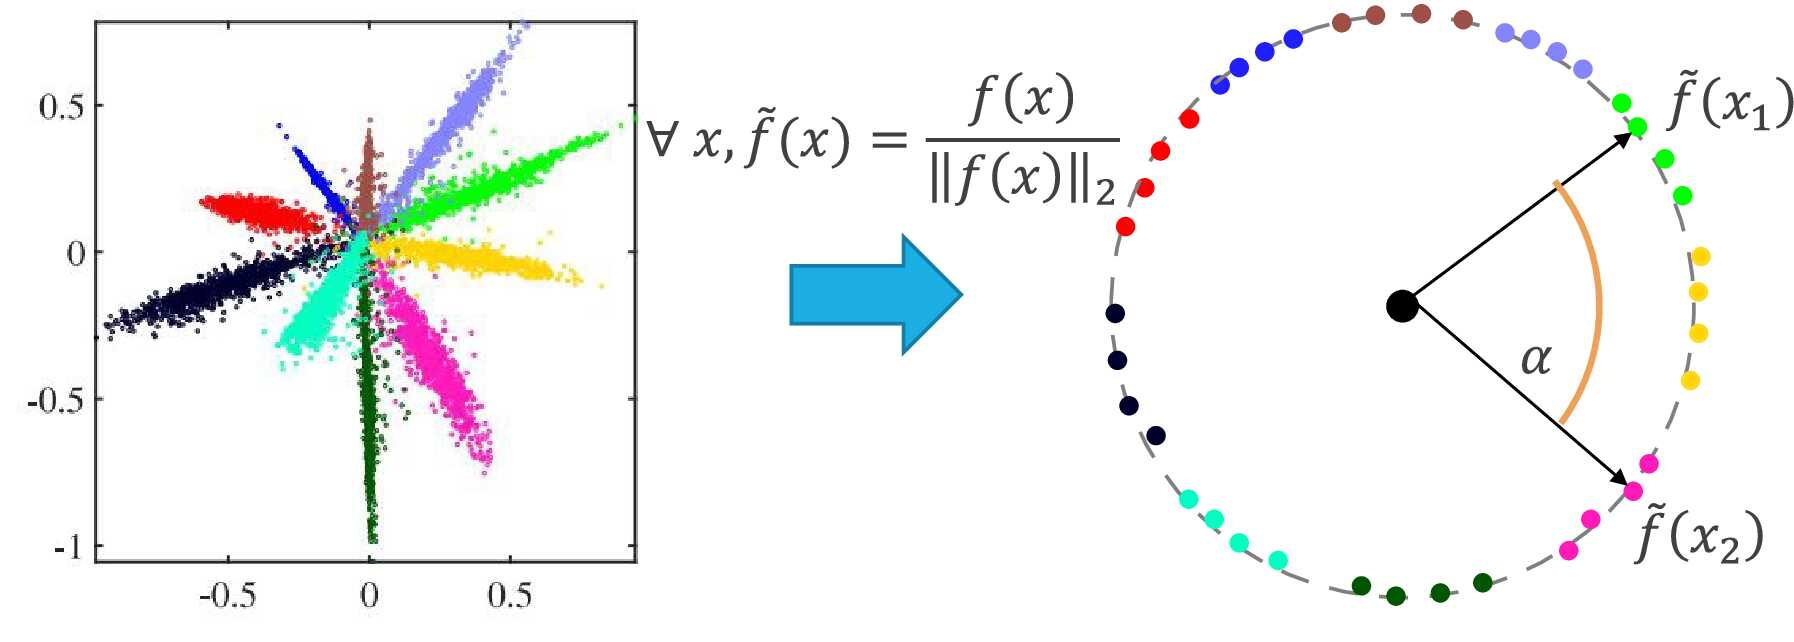
\includegraphics[width=0.6\linewidth]{./img/_embedding_l2_norm_effect.jpg}
    \end{figure}
\end{remark}

\begin{remark}
    With normalized embeddings, classification with softmax as pre-training objective becomes more reasonable. The advantage with softmax is that it does not require sampling informative negative examples. However, as is, it is unable to identify well separated cluster.
\end{remark}

\begin{remark}[Recall: linear classifiers]
    A linear classifier is equivalent to performing template matching. Each column of the weight matrix represents a template.

    \begin{figure}[H]
        \centering
        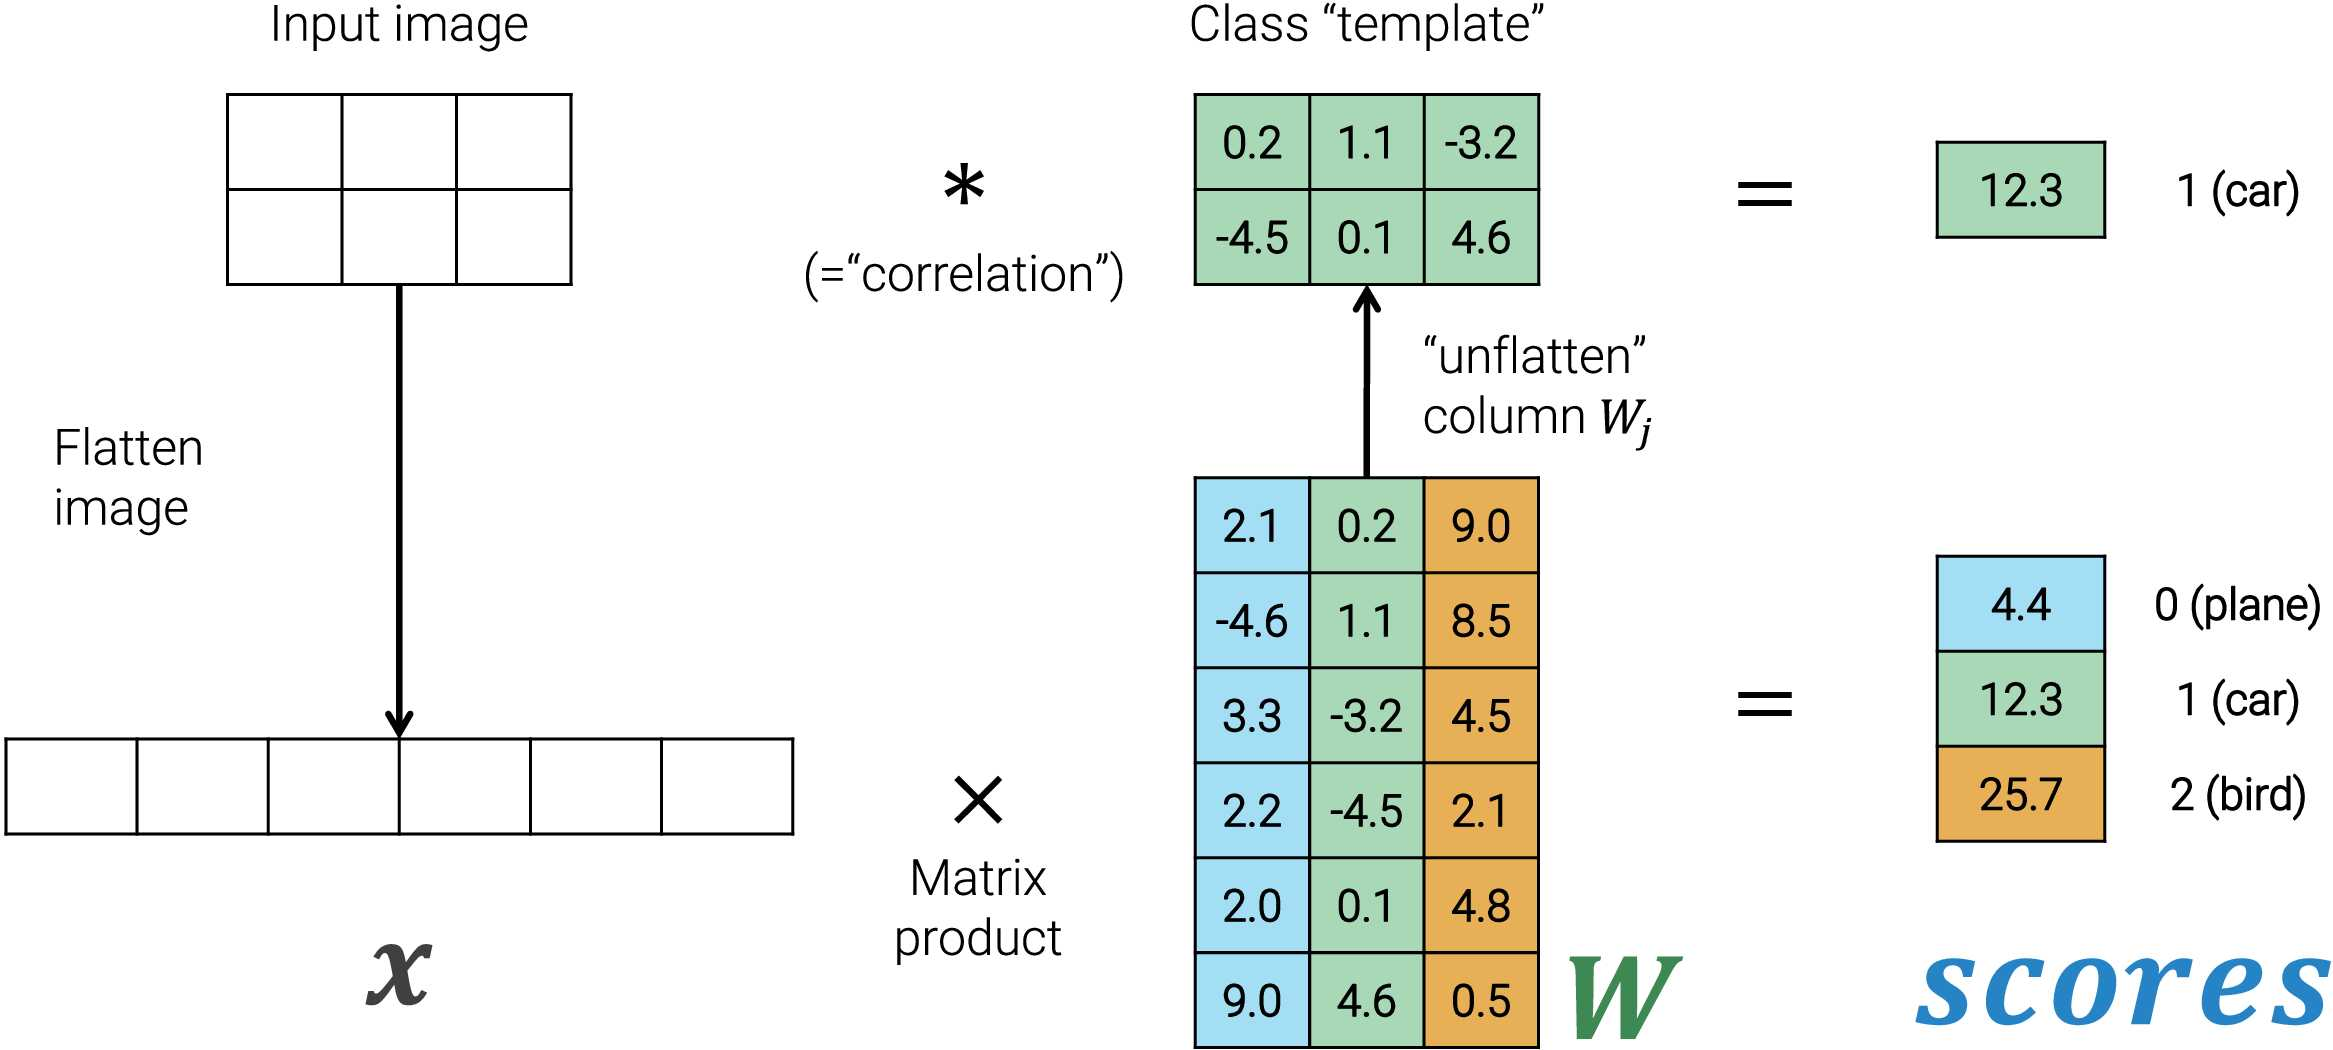
\includegraphics[width=0.6\linewidth]{./img/_template_matching.jpg}
    \end{figure}
\end{remark}

\begin{description}
    \item[ArcFace loss] \marginnote{ArcFace loss}
        Modification to softmax to enforce clustered classes.

        Consider a classification head with a linear layer added on top of the embedding model during training. The weight matrix $\matr{W}$ of the linear layer has a column for each identity. If $\matr{W}$ is L2 normalized ($\tilde{\matr{W}}$), applying the linear layer is equivalent to computing the cosine similarity between the embedding and each identity template. 

        \begin{figure}[H]
            \centering
            \begin{subfigure}{0.48\linewidth}
                \centering
                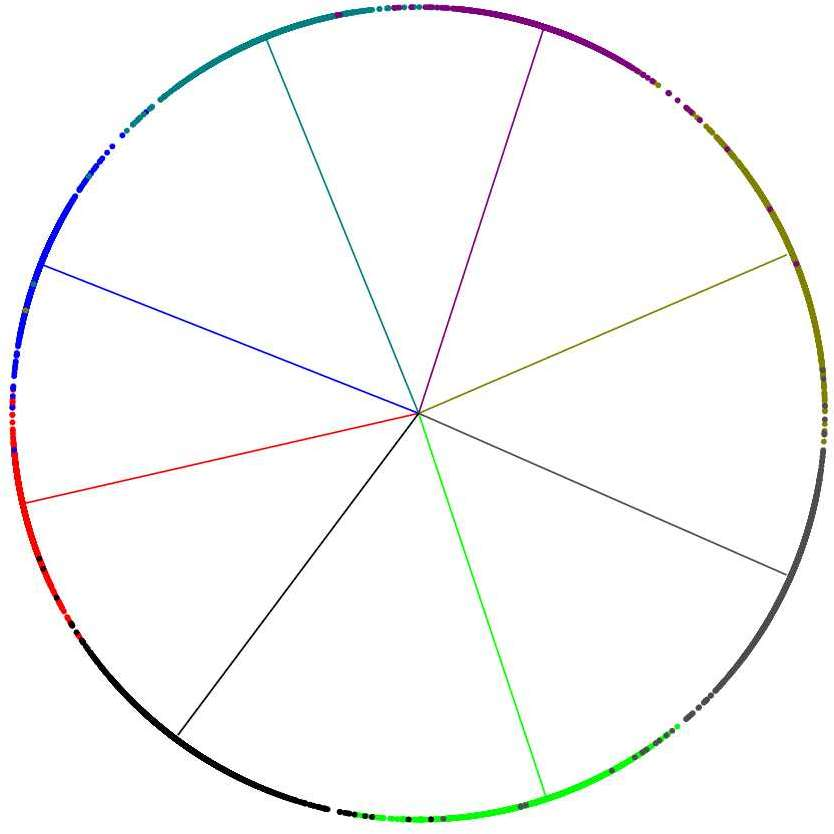
\includegraphics[width=0.5\linewidth]{./img/_arcface_softmax.jpg}
                \caption{Softmax}
            \end{subfigure}
            \begin{subfigure}{0.48\linewidth}
                \centering
                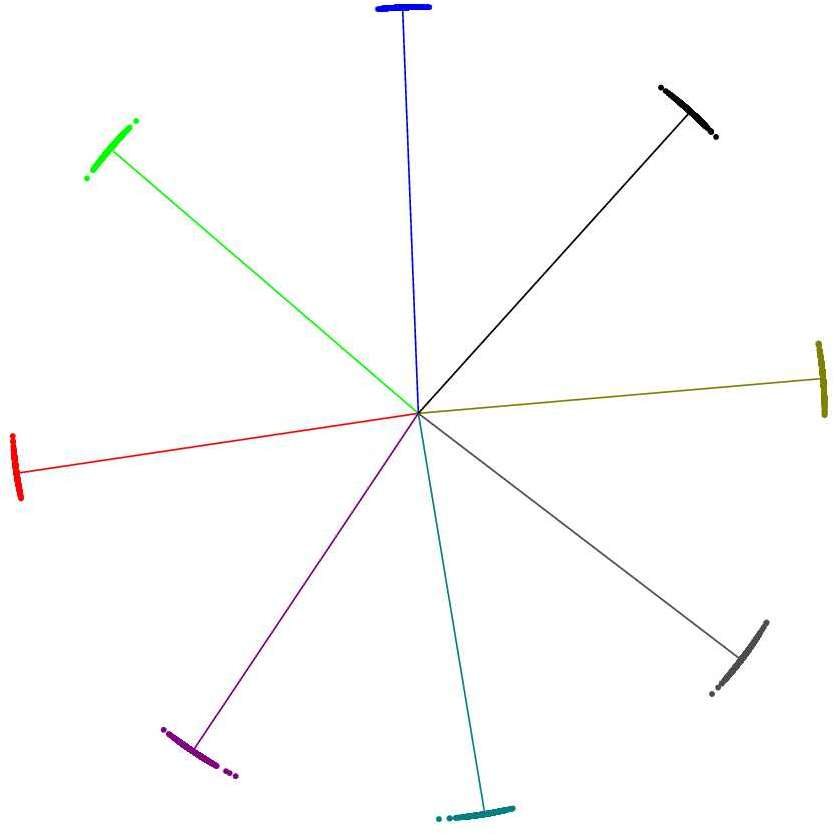
\includegraphics[width=0.5\linewidth]{./img/_arcface_cluster.jpg}
                \caption{ArcFace}
            \end{subfigure}
            \caption{
                \parbox[t]{0.7\linewidth}{
                    Classification results with L2 normalized embeddings. Points represent embeddings and colors are the classes. The points marked by the radii are the templates. Note that with softmax there is no clear distinction between identities.
                }
            }
        \end{figure}

        To enforce that the embedding must be closer to the correct template, the logit $\vec{s}_y$ of the true identity $y$ can be modified with a penalty $m$:
        \[ \vec{s}_y = \cos\left( \arccos(\langle \tilde{\matr{W}}_y, \tilde{f}(x) \rangle) + m \right) \]
        Intuitively, the penalty makes softmax ``think'' that the error is bigger than what it really is, making it push the embedding closer to the correct template.

        \begin{figure}[H]
            \centering
            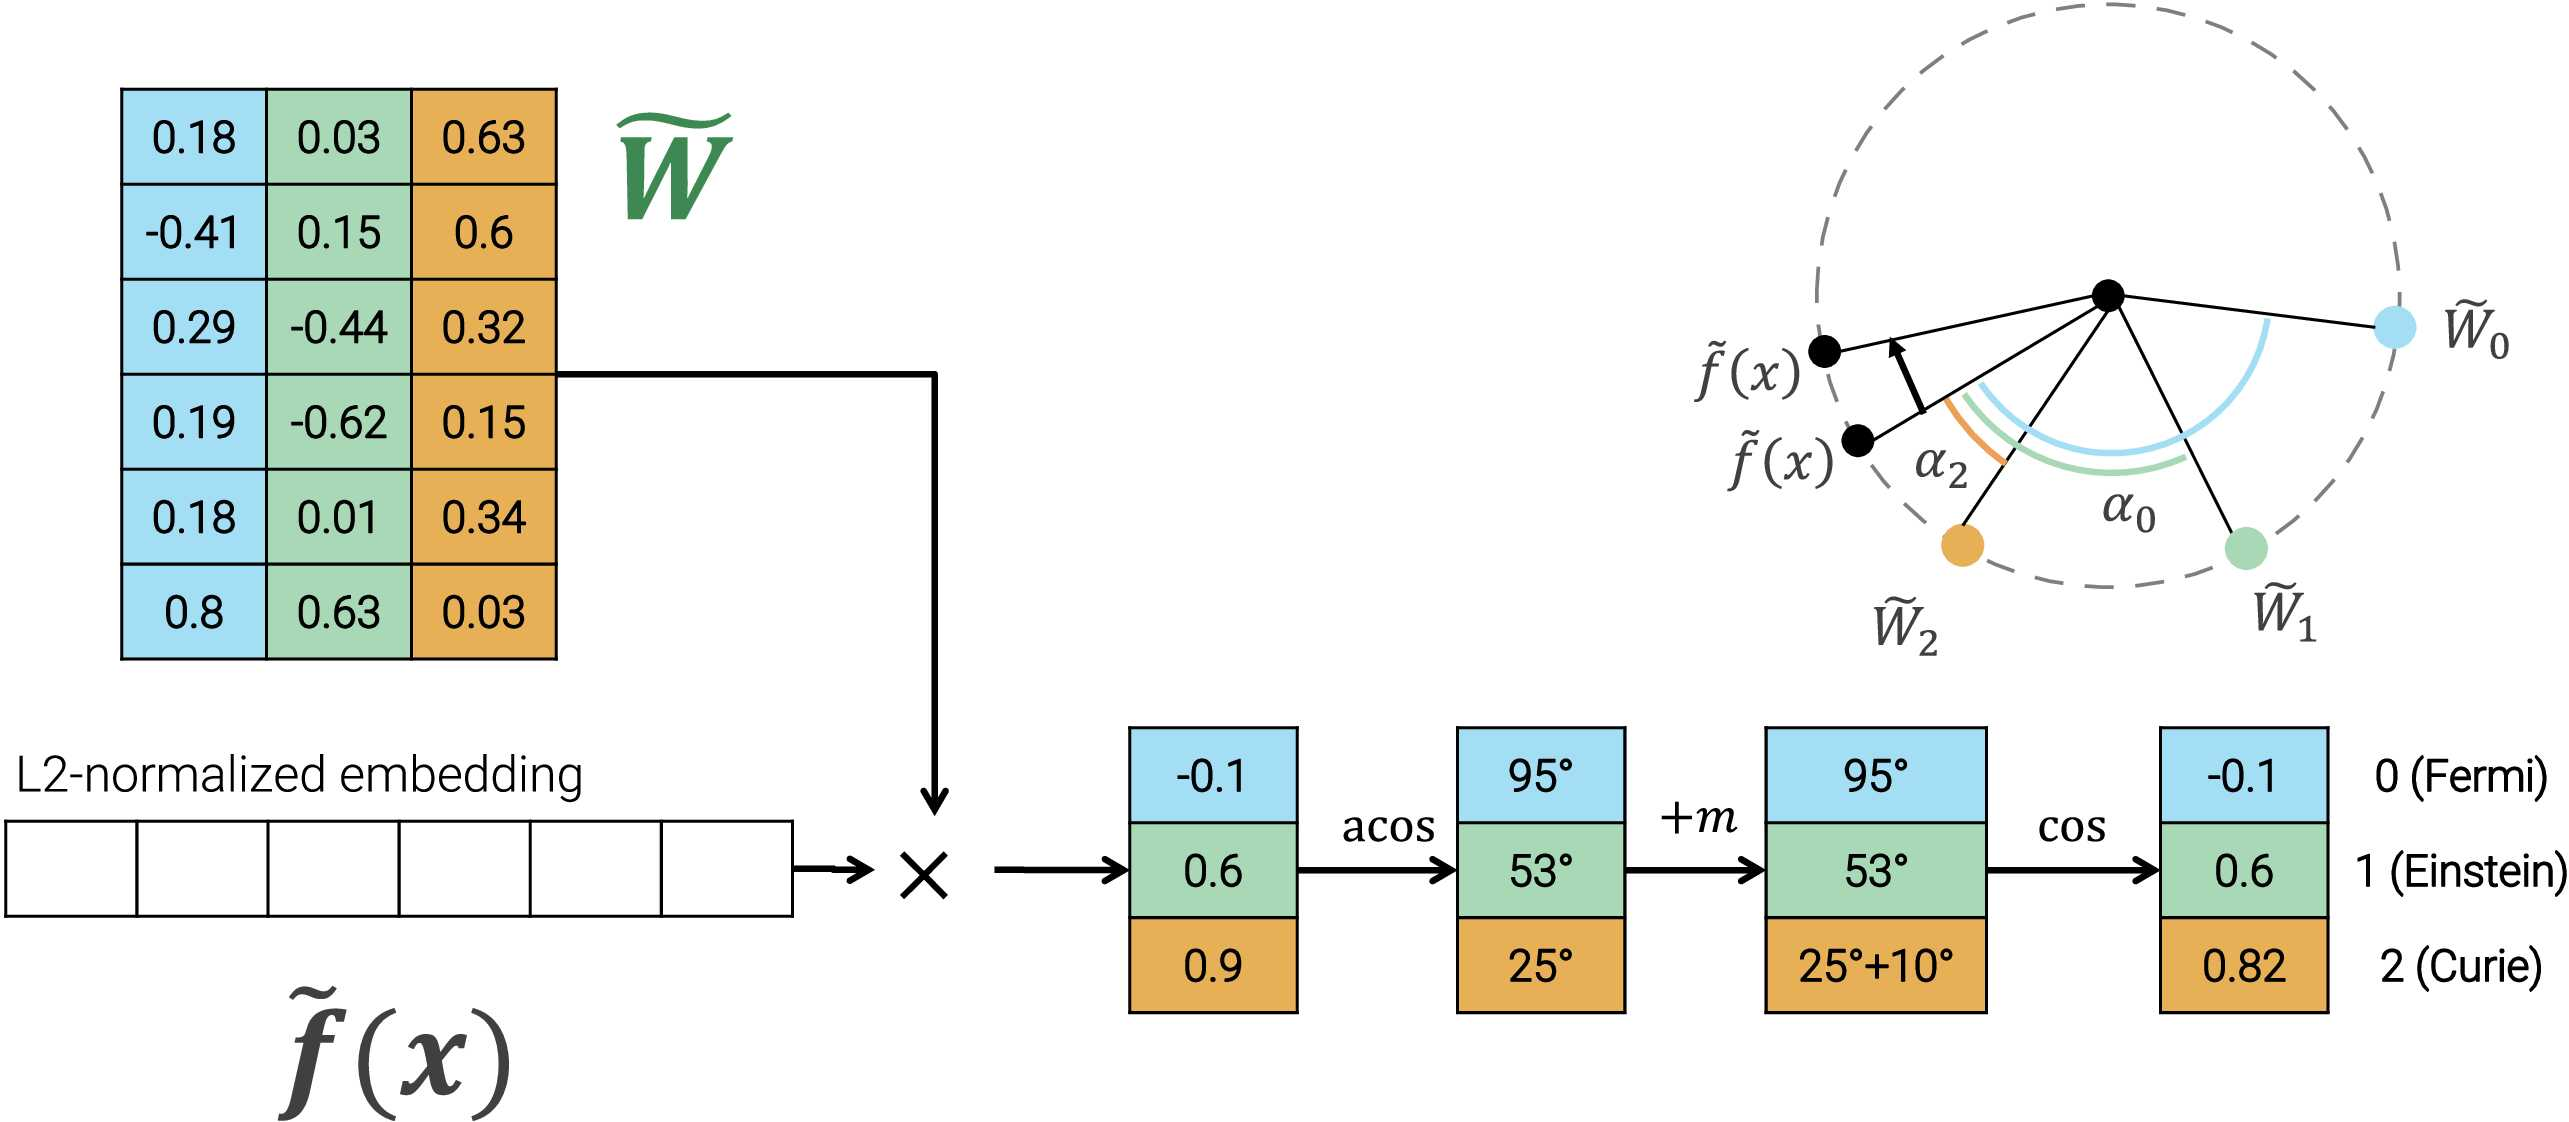
\includegraphics[width=0.65\linewidth]{./img/_arcface_penalty.jpg}
            \caption{Penalty application with \texttt{Curie} as the correct class}
        \end{figure}

        \begin{figure}[H]
            \centering
            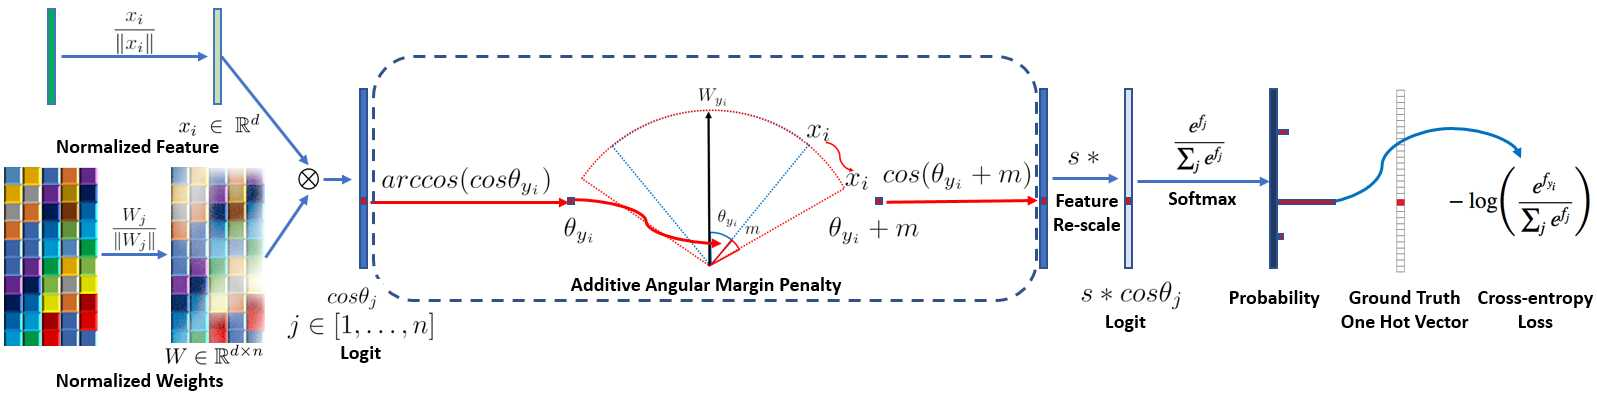
\includegraphics[width=0.95\linewidth]{./img/_arcface_flow.jpg}
            \caption{Overall ArcFace flow}
        \end{figure}
\end{description}


\subsection{NT-Xent / N-pairs / InfoNCE loss}

\begin{description}
    \item[Angular triplet loss] \marginnote{Angular triplet loss}
        Consider the triplet loss (without margin) defined in \Cref{sec:triplet_loss} rewritten in angular form:
        \[ \mathcal{L}_\text{angular\_triplet}(A, P, N) = \max \left\{ 0, \tilde{f}(A)^T \tilde{f}(N) - \tilde{f}(A)^T \tilde{f}(P) \right\} \]

        To avoid the need of sampling negatives, it is possible to consider all of them in the optimization process as follows:
        \[ 
            \begin{split}
                \mathcal{L}&_\text{$n+1$-tuples}(A, P, N_1, \dots, N_n) \\
                &= \max \left\{ 
                    0, 
                    \left(\tilde{f}(A)^T \tilde{f}(N_1) - \tilde{f}(A)^T \tilde{f}(P)\right),
                    \dots,
                    \left(\tilde{f}(A)^T \tilde{f}(N_n) - \tilde{f}(A)^T \tilde{f}(P)\right)
                \right\} 
            \end{split}
        \]

        \begin{remark}
            Backpropagating \texttt{max} considers the gradient of the maximally violating triplet only (i.e., the hardest one which, as seen, is not ideal).
        \end{remark}
\end{description}

\begin{remark}[Recall: cross-entropy with softmax]
    When minimizing cross-entroy with softmax, the loss for a single sample is computed as:
    \[ 
        -\log\left( \frac{ \exp(\vec{s}_{y^{(i)}}) }{\sum_{k=1}^{C} \exp(\vec{s}_k)} \right) =
        - \vec{s}_{y^{(i)}} + \log\left( \sum_{k=1}^{C} \exp(\vec{s}_k) \right)
    \]
    The term $\log( \sum_{k=1}^{C} \exp(\vec{s}_k) )$ is known as the \texttt{logsumexp} and it is usually approximated as the \texttt{max} of the logit:
    \[ \log \left( \sum_{k=1}^{C} \exp(\vec{s}_k) \right) \approx \max_k \vec{s}_k \]
    Or, seen on the other side, \texttt{logsumexp} is an approximation of \texttt{max}.
\end{remark}

\begin{description}
    \item[N-pairs/InfoNCE loss] \marginnote{N-pairs/InfoNCE loss}
        Use the \texttt{logsumexp} as an approximation of \texttt{max} so that all negatives contribute to the gradient step:
        \[
            \footnotesize
            \begin{split}
                \mathcal{L}_\text{InfoNCE}(A, P, N_1, \dots, N_n) &= \texttt{logsumexp}\left( 0, 
                \left(\tilde{f}(A)^T \tilde{f}(N_1) - \tilde{f}(A)^T \tilde{f}(P)\right),
                \dots, \left(\tilde{f}(A)^T \tilde{f}(N_n) - \tilde{f}(A)^T \tilde{f}(P)\right) \right) \\
                &= \log\left( e^0 + \sum_{i=1}^{n} \exp\left(\tilde{f}(A)^T\tilde{f}(N_i) - \tilde{f}(A)^T\tilde{f}(P)\right) \right) \\
                &= \log\left( 1 + \exp\left(-\tilde{f}(A)^T\tilde{f}(P)\right) \sum_{i=1}^{n} \exp\left(\tilde{f}(A)^T\tilde{f}(N_i)\right) \right) \\
                &= \log\left(
                    \frac{\exp\left( \tilde{f}(A)^T\tilde{f}(P) \right)}{\exp\left( \tilde{f}(A)^T\tilde{f}(P) \right)}
                    \left[1 + \exp\left(-\tilde{f}(A)^T\tilde{f}(P)\right) \sum_{i=1}^{n} \exp\left(\tilde{f}(A)^T\tilde{f}(N_i)\right) \right] 
                    \right) \\
                &= \log\left( \frac{\exp\left( \tilde{f}(A)^T\tilde{f}(P) \right) + \sum_{i=1}^{n} \exp\left(\tilde{f}(A)^T\tilde{f}(N_i)\right)}{\exp\left( \tilde{f}(A)^T\tilde{f}(P) \right)} \right) \\
                &= -\log\left( \frac{\exp\left( \tilde{f}(A)^T\tilde{f}(P) \right)}{\exp\left( \tilde{f}(A)^T\tilde{f}(P) \right) + \sum_{i=1}^{n} \exp\left(\tilde{f}(A)^T\tilde{f}(N_i)\right)} \right) \\
            \end{split}
        \]

        \begin{remark}
            In the literature, this loss is known as N-pairs (2016) or InfoNCE (2018).
        \end{remark}

    \item[NT-Xent loss] \marginnote{NT-Xent loss}
        Add a temperature $\tau$ to N-pairs/InfoNCE loss so that more negatives are relevant when backpropagating:
        \[ 
            \small
            \mathcal{L}_\text{NT-Xent}(A, P, N_1, \dots, N_n) =
            -\log\left( \frac{\exp\left( \frac{\tilde{f}(A)^T\tilde{f}(P)}{\tau} \right)}{\exp\left( \frac{\tilde{f}(A)^T\tilde{f}(P)}{\tau} \right) + \sum_{i=1}^{n} \exp\left(\frac{\tilde{f}(A)^T\tilde{f}(N_i)}{\tau}\right)} \right)
        \]

        \begin{remark}
            This loss is sometimes identified as the contrastive loss.
        \end{remark}
\end{description}

\begin{remark}
    Empirical studies found out that the different metric learning losses all perform similarly with fixed hyperparameters while avoiding test set feedback (i.e., avoid leaking test data into training).
\end{remark}


% \begin{description}
%     \item[GrokNet]
% \end{description}


\section{Zero-shot classification}

\begin{description}
    \item[Zero-shot classification] \marginnote{Zero-shot classification}
        Classify images from the test set of a dataset without training on its training set.

        \begin{remark}
            Natural language supervision works well for zero-shot classification by connecting the representation of images and texts. An easy way to obtain image-text pairs is to use the \texttt{alt} tag of HTML images (i.e., the description of the image used by screen readers).
        \end{remark}
\end{description}


\subsection{Contrastive language-image pre-training (CLIP)}

\begin{description}
    \item[Contrastive language-image pre-training (CLIP)] \marginnote{Contrastive language-image pre-training (CLIP)}
        Network composed of:
        \begin{descriptionlist}
            \item[Text encoder] 
                Transformer encoder where the \texttt{[EOS]} token is used as the representation of the sequence.

            \item[Image encoder] 
                ResNet with global average pooling or ViT where the \texttt{[CLS]} token is used as representation.
        \end{descriptionlist}
        A linear projection is used to match the shapes of the two encoders.

        \begin{description}
            \item[Training] 
                Given a batch of text-image pairs $(t_1, i_1), \dots, (t_N, i_N)$, texts and images are processed by their respective encoders. The embeddings $T_j$, $I_j$ are then compared pairwise: text and image embeddings corresponding to the same entity are considered a positive class, otherwise, they represent a negative class.
                NT-Xent loss is computed across the images by fixing a text or vice versa.

                \begin{figure}[H]
                    \centering
                    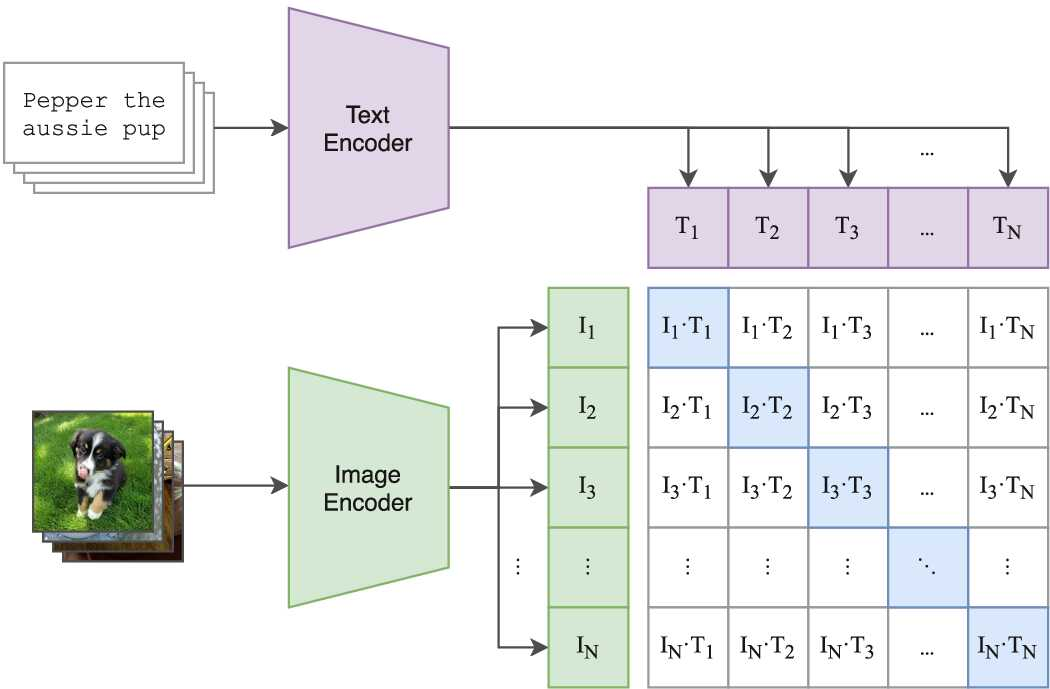
\includegraphics[width=0.6\linewidth]{./img/_clip_training.jpg}
                    \caption{
                        \parbox[t]{0.6\linewidth}{CLIP training flow. NT-Xent loss is applied column or row-wise in the dot product matrix.}
                    }
                \end{figure}

                \begin{remark}
                    It has been seen that as bag-of-words approach for the text encoder is better than using transformers.
                \end{remark}

                \begin{remark}
                    As the NT-Xent loss is used, a large batch size is used.
                \end{remark}

                \begin{remark}
                    CLIP with ViT-L/14 is the ``standard'' version. It has been pre-trained for an additional epoch on images with a higher resolution, similarly to FixRes (i.e., deal with different train and test resolutions).
                \end{remark}

            \item[Inference]
                Given an image to classify, it is embedded and compared with the embeddings of prompts referencing the classes (e.g., \texttt{a photo of a [object]}). The closest one is considered as the predicted class.
                \begin{figure}[H]
                    \centering
                    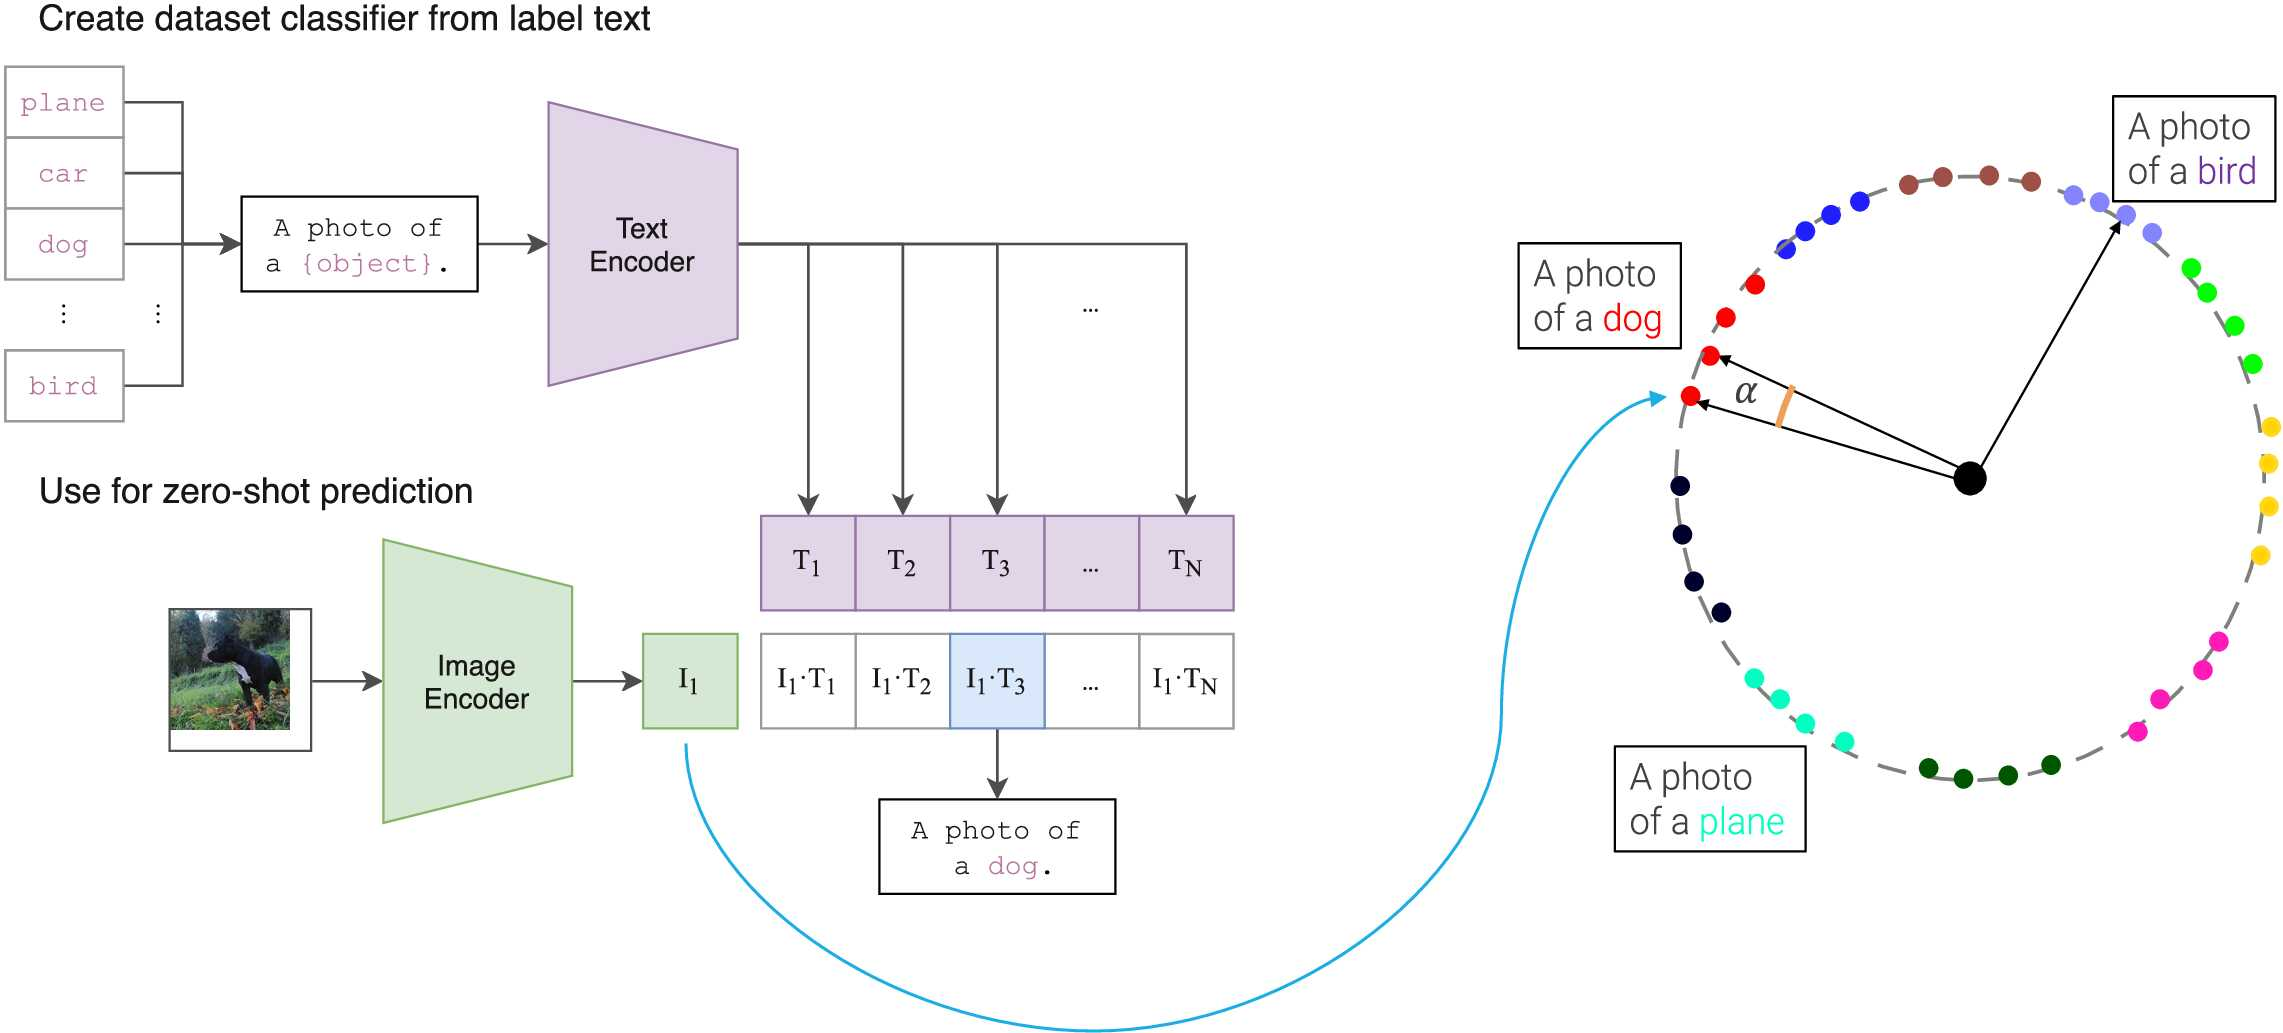
\includegraphics[width=0.85\linewidth]{./img/_clip_inference.jpg}
                \end{figure}
        \end{description}

        \begin{remark}
            CLIP features are robust to distribution shifts (i.e., the network does not take ``shortcuts'' when classifying).

            \indenttbox
            \begin{example}
                As lesions in x-ray images are marked by the doctors, a network trained to detect lesions might actually learn to predict the mark put by the doctors.
            \end{example}

            \begin{figure}[H]
                \centering
                \begin{subfigure}{0.35\linewidth}
                    \centering
                    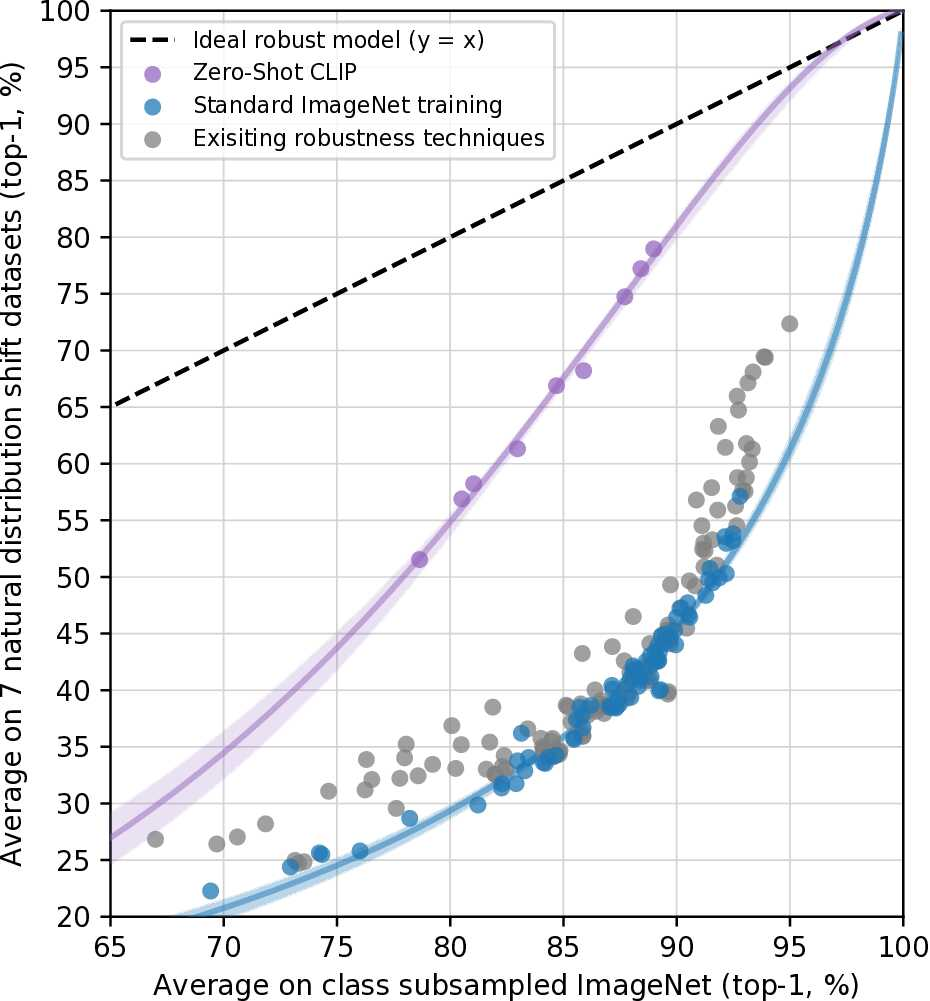
\includegraphics[width=\linewidth]{./img/_clip_resnet_distributional_shift.jpg}
                \end{subfigure}
                \hfill
                \begin{subfigure}{0.6\linewidth}
                    \centering
                    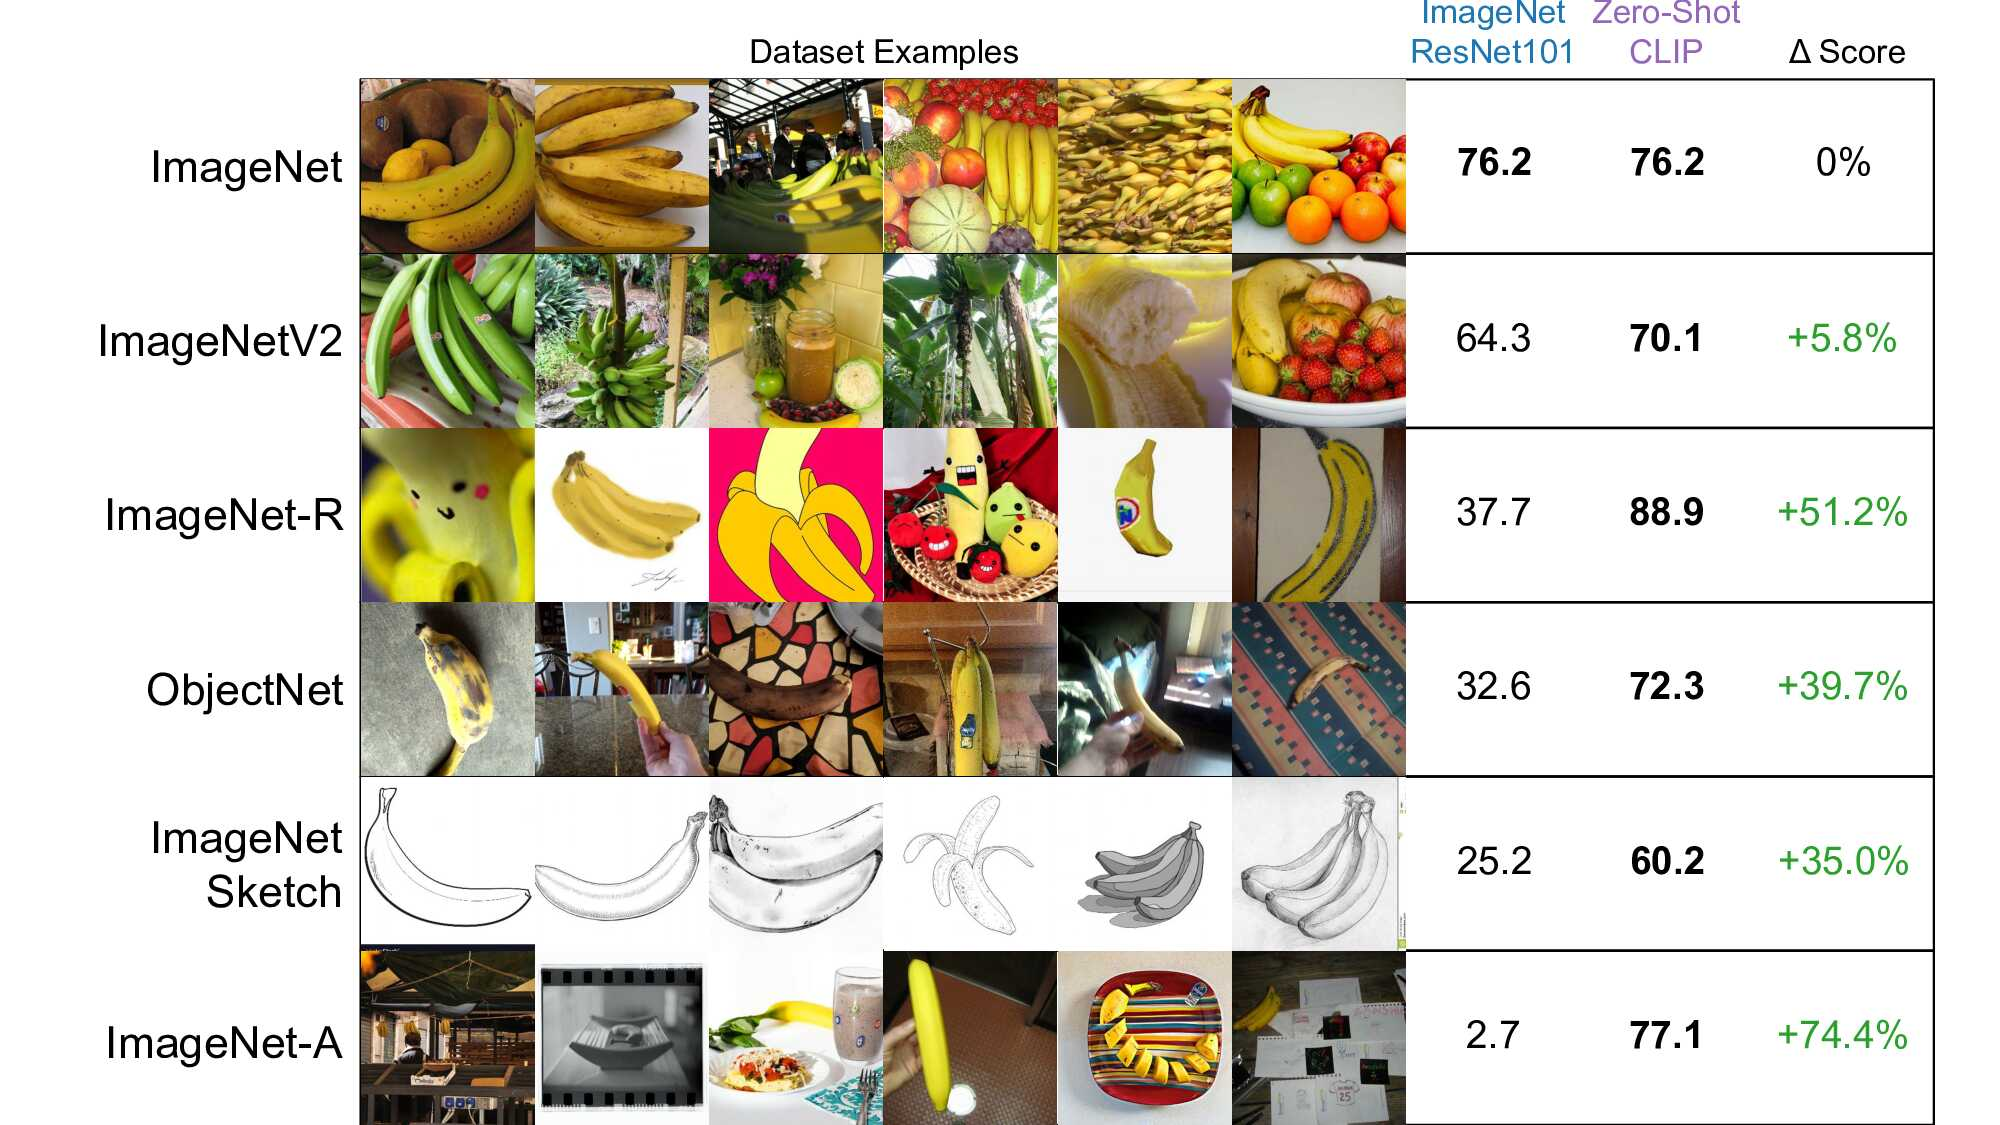
\includegraphics[width=\linewidth]{./img/_clip_resnet_distributional_shift_datasets.jpg}
                \end{subfigure}
            \end{figure}
        \end{remark}
\end{description}

\begin{remark}[CLIP for text-conditioned generative models]
    CLIP can be used as a loss for a generative model to condition generation based on a prompt. Given a desired prompt, the steps are the following:
    \begin{enumerate}
        \item Freeze both the generator and CLIP.
        \item Feed the generator a random input $z$ to generate an image.
        \item Embed the generated image with CLIP and compare it to the embedding of the prompt.
        \item Gradient ascent is used to improve $z$ aiming to maximize the similarity.
    \end{enumerate}

    \begin{figure}[H]
        \centering
        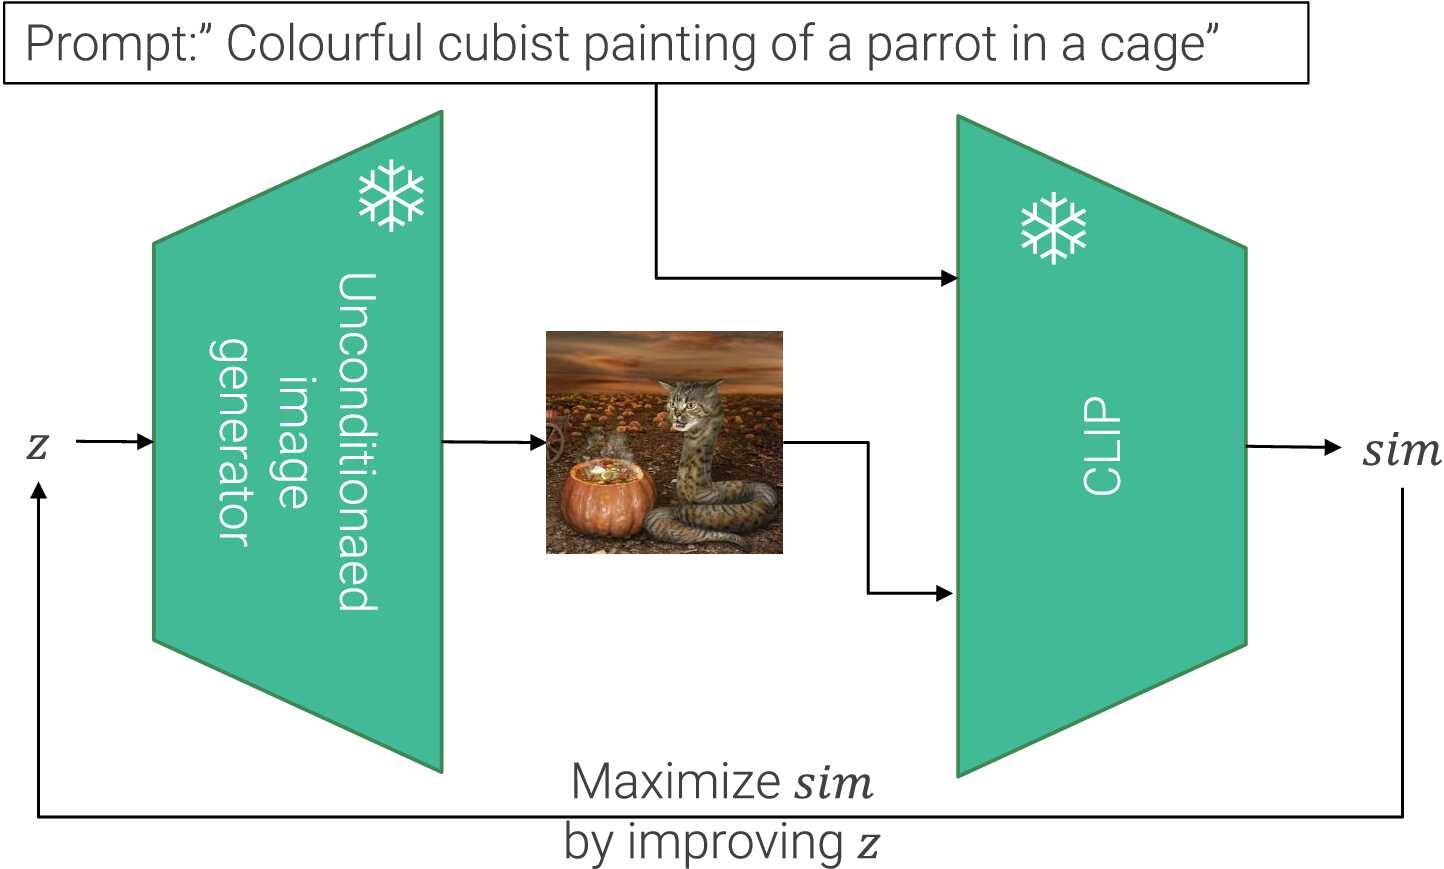
\includegraphics[width=0.5\linewidth]{./img/_clip_generation_conditioning.jpg}
    \end{figure}
\end{remark}